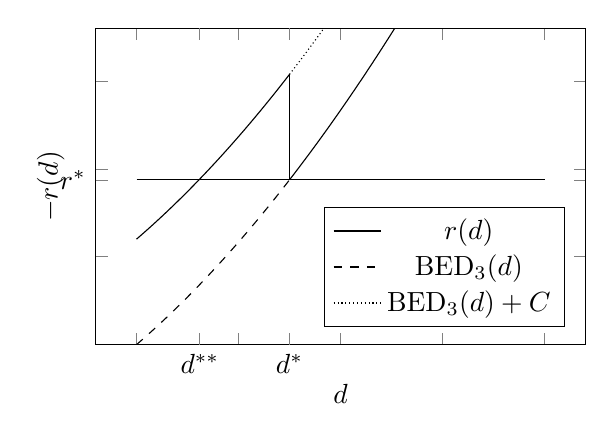
\begin{tikzpicture}
    \begin{axis}
    [
        ymin=0,
        ymax=1.8,
        xlabel={$d$}, 
        ylabel={$-r(d)$},
        ylabel style=
        {
        yshift=-3mm
        },
        xlabel style=
        {
        yshift=+1mm
        },
        yticklabels={,,},
        xticklabels={,,},
%        ticks=none,
        legend style={at={(axis cs:2.1,0.1)}, anchor=south east},
        width=7.8cm,
        height=5.6cm,
        extra y ticks={0.9375},
        extra y tick labels={$r^{*}$},
        extra x ticks={0.31, 0.75},
        extra x tick labels={$d^{**}$, $d^{*}$}
    ]
    
    \addplot[no marks, solid, domain=0:0.75, samples=50] {x + ((x^2)/3) + 0.6};
    \addlegendentry{$r(d)$}
    
    \addplot[no marks, dashed, domain=0:0.75, samples=50] {x + ((x^2)/3)};
    \addlegendentry{BED$_3(d)$}
    
    \addplot[no marks, densely dotted, domain=0.75:2, samples=50] {x + ((x^2)/3) + 0.6};
    \addlegendentry{BED$_3(d) + C$}
    
    \addplot[no marks, solid, domain=0.75:2, samples=50] {x + ((x^2)/3)};
    
    \addplot[no marks, solid, domain=0:2, samples=50] {x*0 + 0.9375};
    
    \addplot [no marks, solid, domain=0:1, samples=50]
        coordinates {(0.75,0.9375)(0.75,1.5375)};
    
    \end{axis}
\end{tikzpicture}